\section{Recent Research Progress}
Our work over the last four years has described, at nucleotide resolution, the chromatin occupancy dynamics associated with the initiation of DNA replication\citep{}, gene expression in response to an environmental stress\cite{}, DNA repair by non-homologous end joining\citep{}, and the re-assembly of chromatin behind the replication fork\citep{}.  

\ssheading{Helicase activation in the absence of DNA replication}
To investigate the transient chromatin changes that occur at origins of DNA replication during initiation, we generated a conditional allele of POL1(CDC17) that blocked replication priming at the non-permissive conditions.  At the onset of S-phase, in the absence of priming, the Cdc45-Mcm2-7-GINS holohelicase (CMG) complex became active and proceeded to unwind origin proximal DNA and disrupt chromatin organization for approximately 1 kb surrounding each activated origin. The CMG helicase stalled at sequences with elevated GC-content suggesting that a functional replisome is required for processivity. A consequence of activating the CMG helicase in the absence of priming is that the origin DNA between the stalled helicases may re-anneal to form duplex DNA and that once priming is restored the stalled CMG helicases are oriented to progress away from the origin potentially leaving un-replicated gaps in their wake. Consistent with this hypothesis, we found that cells are able to recover from the restrictive conditions, but experience a prolonged delay in G2/M and reduced copy number at replication origins. Ultimately, the cells are viable and fully recover suggesting that there are mechanisms to resolve these unreplicated lesions.  

\ssheading{Origin chromatin dynamics through multiple cell cycles}
We generated genome-wide chromatin occupancy profiles for synchronized yeast cells as they progressed through two complete cell cycles.  With ten minute resolution we were able to visualize the chromatin occupancy dynamics at origins and the sequences surrounding origins as they progressed through consecutive cell cycles.  We were able to observe the downstream re-positioning of the +1 nuclesome flanking origins and an increase in protected fragments corresponding to assembly of the pre-replicative complex in G1.  Models for origin efficiency have included the strength of ORC binding, the numbers of Mcm2-7 loaded at origins and the rate limiting concentrations of origin firing components.  In an unbiased manner, we found that strongest correlation between chromatin occupancy at the ACS and origin efficiency occurred in early S-phase with the formation of the Cdc45-Mcm2-7-GINS (CMG) complex supporting the role of rate limiting factors in establishing the replication program.  

\ssheading{Modeling gene expression from chromatin occupancy data}
We have had a long standing collaboration with Dr. Alex Hartemink (Duke) to model gene expression from changes in chromatin occupancy. We used exposure to the heavy metal cadmium to induce a stress response in yeast cells and simultaneously captured chromatin occupancy and gene expression data. We were able to identify chromatin based signatures for transcriptional activation or repression from occupancy differences in nucleosomes and or DNA binding factors\citep{}. We were able to generate predictive models from the chromatin occupancy signatures that rivaled models based on chromatin modification data.  We also developed RoboCOP, a multivariate state space model that integrates chromatin accessibility data (MNase-seq, ATAC-seq, DNase-seq) and sequence, to jointly compute a robust probability estimate for nucleosome and transcription factor occupancy\citep{}. 

\ssheading{Chromatin assembly behind the replication fork}
We developed nascent chromatin occupancy profiling to assess the spatiotemporal dynamics of chromatin assembly at nucleotide resolution behind the DNA replication fork.  Every cell division, the complex regulatory landscape that defines the epigenetic state of the cell must be disassembled and re-assembled in the wake of the replication fork.  We identified locus specific differences in the assembly and maturation of chromatin behind the fork with the histone variant H2A.Z being predictive of genes with rapid maturation kinetics.   We also observed differential chromatin assembly kinetics at replication origins depending on if they underwent initiation or were passively replicated by forks from distal origins. Finally, we found that some DNA binding proteins were transiently associated with nascent chromatin following passage of the fork and which may ultimately contribute to gene regulation.

\ssheading{Chromatin dynamics associated with double-strand break and repair}
We investigated the chromatin dynamics following induction of a site specific double-strand break and the subsequent repair of the break by non-homologous end joining (NHEJ).  We found that the nucleosomes flanking the break were immediately evicted in an mre11-dependent manner and that nucleosomes more distal to the break were translocated away from the site of damage unless blocked by a transcription factor.  We allowed the cells to repair the genetic lesion by NHEJ and asked whether the cells were also able to repair the epigenetic lesion (disrupted nucleosome organization) or did they require passage through S-phase.  We found that S-phase was not required to restore the precise nucleosome organization at the repaired lesion and that there must exist replication independent chromatin assembly mechanisms to restore the epgienetic landscape at sites of DNA damage and repair.


\ssheading{Collaborative work}
We have been fortunate to participate in a number of exciting collaborations based, in part, on our expertise in molecular biology, genomics and DNA replication.  In collaboration with Dr. Chris Counter (Duke) we used our expertise in molecular biology to develop and extend maximum depth sequencing\cite{} to mammalian genomes.  Using maximum depth sequencing we were able to identify initiating oncogenic mutations in RAS alleles with extreme sensitivity (~1 mutant/million templates) immediately following treatment with a carcinogen\cite{}.  Together with Dr. Robert Duronio (UNC) we characterized the replication timing of sequences throughout the Drosophila genome from developing wing imaginal disc cells and the role of repressive chromatin marks (H3K9me3) in establishing the late DNA replication program\citep{}.  Using Drosophila histone gene engineering\citep{} we were able to replace lysine 9 on histone h3 with an arginine (H3K9R).  The resulting H3K9R flies exhibited decreased hp1a and increased accessibility and transcription in the pericentric heterochromatin chromatin, but the majority of pericentric heterochromatin remained late replicating, suggesting that sequence features may be more predictive of late replication than epigenetic features.  Finally, with Antonio Bedalov (FHCRC) we were able to demonstrate that active transcription of a RNA pol II non-coding transcript at the rDNA was able to push and relocalize the Mcm2-7 complex away from their initial loading site into a region of decreased nucleosome occupancy.  The relocalization of the helicase by the transcription machinery resulted in increased rDNA origin efficiency.  This work supports prior work from our group\citep{} and the Remus lab\citep{} demonstrating  plasticity in origin selection by transcription mediated displacement of the mcm2-7 helicase. 



% %letters from danny, iystin. hartemink









% Chromatin assembly
% DNA repair
% helicase activation
% Chromatin regulation of gene expression
% Collaborative

% \section{Future Research Directions}
% Single molecule DMSO m6A absent in yeast -- characterize single reads. 

% DNA repair 
% NHEJ -- strand specific labeling HR; BIR 

% Chromatin assembly
% Chromatin assembly behind the replication fork (interogating at locus specific resolution -- advance strand specific libraries.  Fast and slow nucleosomes; txp; chaperones; strand specific data.

% Completion of un-replicated DNA

% Transcription
% Chromatin regulation of gene expression -- networks from txp data and deletion data.

% Drosophila letter from whitehouse.  













% \


% \sheading{Chromatin organization and DNA replication in \scer}
% \ssheading{Chromatin architecture of replication origins}
% To better understand how the chromatin environment impacts the selection and regulation of replication origins, we evaluated the DNA occupancy of nucleosomes and the majority of DNA-binding proteins (\eg transcription factors and replication initiation proteins) to generate genome-wide chromatin occupancy profiles (GCOPs)({\color{dukeblue}\textbf{Figure 1}}). Briefly, total chromatin is digested with micrococcal nuclease (MNase) and all of the recovered DNA fragments are subjected to paired-end next-generation sequencing\citep{Belsky2015-li,Henikoff2011-vo}.  Importantly, the size of the sequenced fragment represents whether it was protected by a nucleosome ($\sim$147 bp) or a DNA-binding factor ($<$50 bp). This assay is factor agnostic and reveals specific footprints for more than 70\% of the yeast DNA-binding factors\citep{Henikoff2011-vo}.  Although the assay only provides information about the occupancy state of the DNA, we can often infer the identity of the factor bound from motifs and prior genomic experiments.  
% \begin{floatingfigure}[lt]{2.6in}
% \vspace{-4mm}
% \begin{center}
% 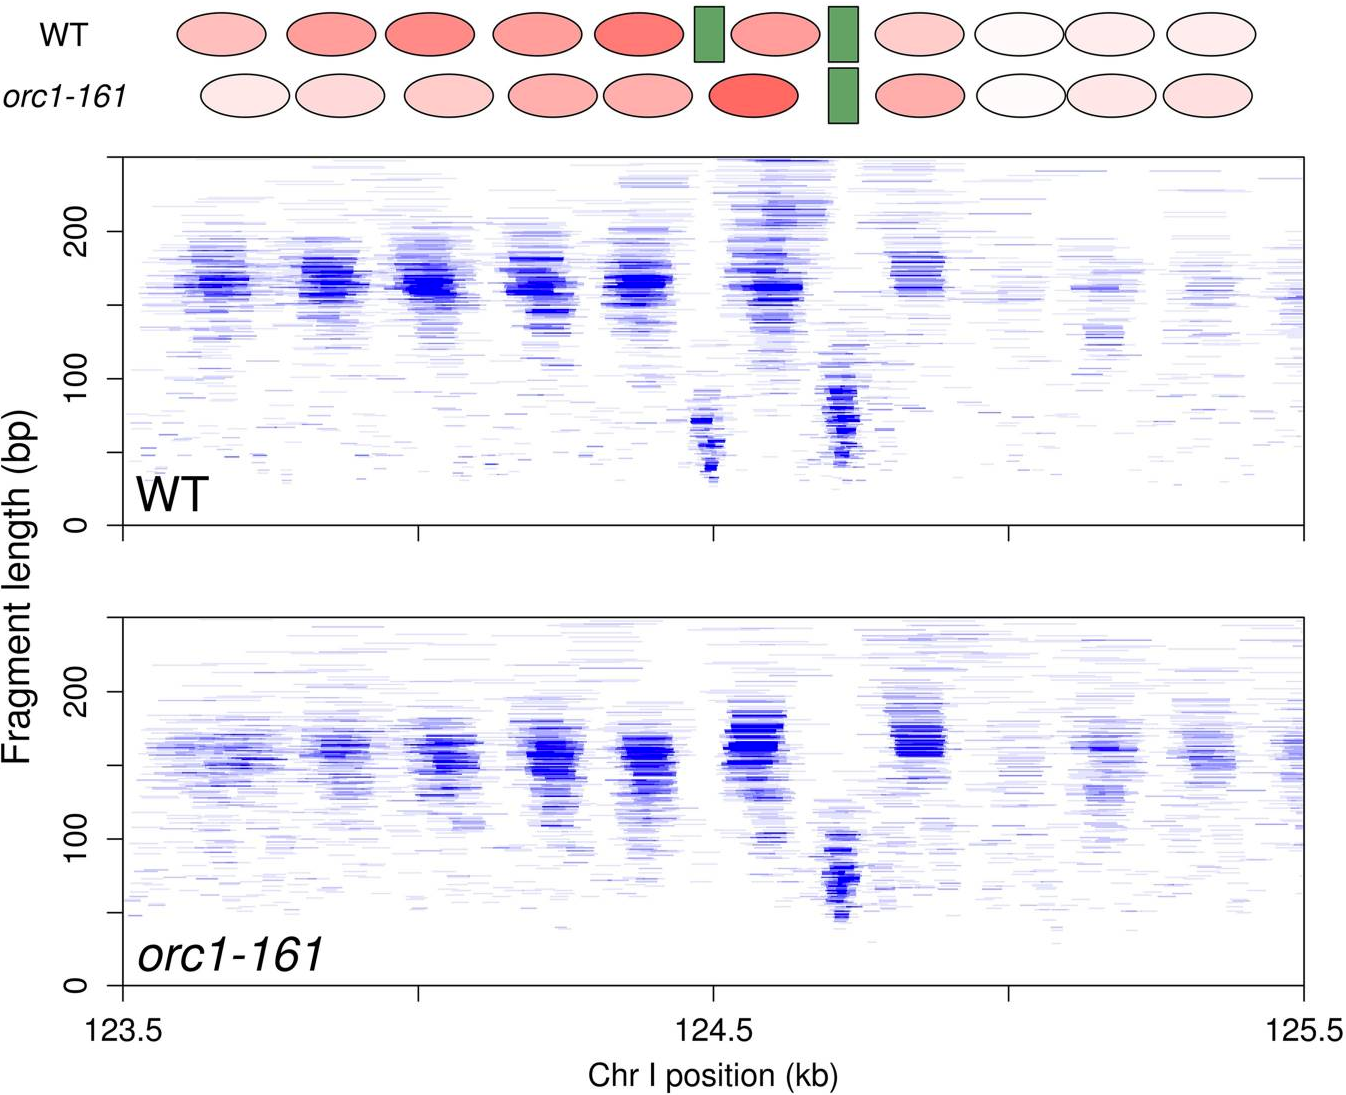
\includegraphics[width=2.6in]{r35_figures/orc_chromatin_gcop.png}
% \end{center}
% \vspace{3mm}
% \caption{GCOP of a replication origin.  MNase protected DNA fragments were subjected to paired-end sequencing and the resulting fragment lengths were plotted as a function of chromosomal position.  Well phased fragments at $\sim$150 bp represent sequences protected by nucleosomes (red ovals in cartoon) and smaller fragments represent other DNA binding factors (\eg ORC at the ACS and Abf1).  In an \textit{ORC1-161} mutant the footprint at the ACS disappears at the non-permissive temperature.}%
% \end{floatingfigure}%
% Our `footprinting' of the \scer genome at distinct cell cycle stages provided the  %the We `footprinted' the \scer\ genome at multiple points in the cell cycle including G2 (ORC alone) and G1 (pre-RC assembly)\citep{Belsky2015-li}.  Together, these experiments provide the 
% following advances and new insights into our understanding of the DNA replication program: i) a novel method to map origins of DNA replication by their ORC-dependent chromatin footprints -- this data provides structural information not only about ORC binding but also the surrounding chromatin and adjacent DNA binding factors at each individual origin; ii) identification of a non-canonical class of inefficient origins that lacked an ORC-dependent footprint in G2, but exhibited a clear footprint in G1 -- the mechanistic implication being that determinants of replication efficiency are established in G2 prior to pre-RC assembly; iii) nucleosome remodeling at the origin is required for efficient origin activation, but not pre-RC assembly -- highlighting the importance of nucleosome dynamics for downstream initiation events including origin unwinding and activation; iv) the loading of a singe Mcm2-7 double hexamer per origin in complex with either the up or downstream flanking nucleosome -- addressing a fundamental question in the field -- where, in relation to ORC, and how many Mcm2-7 double-hexamers are loaded per origin \invivo. 

% Recent work has sought to identify the chromatin remodeling activities responsible for nucleosome dynamics at replication origins.  %We have systematically evaluated all single, double and triple combinations of non-essential chromatin ATP-dependent chromatin remodelers in \scer for their impact on ORC binding, pre-RC assembly and origin activity. While the replication program was surprisingly resistant to loss of ATP-dependent chromatin remodelers, 
% We found that both \textit{ISW1} and \textit{CHD1}  are required for origin activation of inefficient origins (manuscript submitted). In collaboration with Steve Bell (MIT), we have recently demonstrated that the \invitro assembly of nucleosomes by specific chromatin remodeling enzymes can impact pre-RC assembly and initiation in a reconstituted system\citep{Azmi2017-gg}.

% \sheading{DNA replication and maintenance of genome integrity in \dros}
% As a data production center for the model organism ENCODE (modENCODE) project we generated more than one hundred genome-wide datasets describing the \dros replication program\citep{Mod_Encode_Consortium2010-io}.  In the capstone manuscript for the modENCODE project, more than 1400 genomic datasets from modENCODE and ENCODE revealed conserved principles and features of chromatin organization between flies, worms and humans\citep{Ho2014-xa}. %We identified conserved features of chromatin state and genome organization that were linked to the establishment of the DNA replication program. 
% %In addition to the capstone manuscript, we published 12 manuscripts over the course of the project. 
% Below I've highlighted several of our mechanistic follow-up studies in \dros that were supported by our NIGMS-funded R01.

% \ssheading{DNA replication and transcription programs respond to the same epigenetic cues}
% %The a time at which a sequence replicates during S-phase has long been coordinated with transcriptional activity in higher eukaryotes. 
% We and others have correlated gene expression, open chromatin and chromatin modifications with origin location and replication timing data\citep{Rhind2013-yr}.  However, correlation does not  imply causation and due to multiple activating and repressive chromatin modifications it has been difficult to mechanistically assign a direct role to specific chromatin modifications in regulating the DNA replication program. We demonstrated that the early replication of the \dros male X chromosome was dependent on dosage compensation and the male-specific H4K16 hyperacetylation of the X chromosome\citep{Lubelsky2014-zn}.  These results demonstrate that the transcription and DNA replication programs respond to the same epigenetic cues.

% \ssheading{H4K20 monomethylation and genome integrity}
% PR-Set7 is a cell cycle regulated methyl transferase that specifically monomethylates H4K20\citep{Beck2012-uc}.  In mammalian cells, loss of PR-Set7 and the resulting H4K20me1 is associated with delayed S-phase progression and elevated DNA damage presumably due to defects in pre-RC assembly and origin activation\citep{Tardat2010-qc}.  %However, prior studies only examined a handful of mammalian origins and it remained possible that the observed origin specific phenotypes were not due to perturbation of histone methylation, but PR-Set7 mediated methylation of other cell cycle  factors\citep{Shi2007-gz}. 
% Although PR-Set7 is an essential gene in \dros, alanine substitution histone tail mutants (H4K20A) were sick but viable\citep{McKay2015-nn}, arguing that H4K20 methylation is not essential for DNA replication. We found that deregulation of PR-Set7 activity did not impact origin activation in \dros, but rather H4K20 monomethylation was required for maintaining genomic integrity of late replicating domains\citep{Li2016-fi}.  We propose that the accumulation of unmodified H4K20 hinders fork progression through late replicating sequences and results in stochastic replication fork collapse.


% \ssheading{Mcm2-7 Paradox}
% The `MCM Paradox' describes a %long standing 
% series of %seemingly
% paradoxical observations regarding the quantity and location of the Mcm2-7 helicase complex during S-phase in higher eukaryotes\citep{Takahashi2005-bz}. Briefly, there is a vast excess of the Mcm2-7 complexes relative to origins of replication or ORC binding sites, the majority of which are %; %the Mcm2-7 complexes do not appear to localize to ORC by immunofluorescence experiments
% %and the vast majority of the Mcm2-7 complex are 
% dispensable during an unperturbed S-phase. We examined the `MCM Paradox'  using  genomic and biochemical approaches  to understand the mechanisms by which excess Mcm2-7 are loaded and distributed throughout the genome to preserve genomic integrity\citep{Powell2015-af}.  We found that during G1, Mcm2-7 is loaded onto chromatin in two distinct phases -- both of which rely on the canonical pre-RC assembly pathway including Dup/Cdt1 and Cdc6.  In the first phase of pre-RC assembly, a minimal level of Mcm2-7 is loaded specifically at ORC binding sites throughout the genome in a CDK independent manner.  There is also a second wave of pre-RC assembly that is CDK dependent which is required for the loading of the full complement (40 fold increase) of Mcm2-7 onto chromatin.  Strikingly, the full complement of Mcm2-7 is not restricted to sequences immediately adjacent to ORC binding sites, but rather distributed throughout the genome and shaped by active transcription.  %We find that the full complement of Mcm2-7 complex is displaced from actively transcribed regions suggesting that transcription can push or displace the Mcm2-7 complex through gene bodies.  
% %Recent work from the Remus laboratory in \scer  has demonstrated that the Mcm2-7 complex can be pushed away from ORC binding sites by RNA Polymerase \invitro and \invivo resulting in origin activation being displaced from the site of pre-RC assembly\citep{Gros2015-oo}.  Together, 
% These data provide an intriguing model whereby the transcription program may shape the distribution of the Mcm2-7 complex and ultimately origin location which may explain the seemingly random distribution of metazoan origins in higher eukaryotes\citep{Petryk2016-rr}.

